\documentclass{beamer}

\mode<presentation>
{
  \usetheme{CambridgeUS}      % or try Darmstadt, Madrid, ...
  \usecolortheme{default} % or try albatross, beaver, crane, ...
  \usefonttheme{default}  % or try serif, structurebold, ...
  \setbeamertemplate{navigation symbols}{}
  \setbeamertemplate{caption}[numbered]
} 

\usepackage[english]{babel}
\usepackage[utf8x]{inputenc}
\usepackage{listings}
\usepackage[ampersand]{easylist}



\definecolor{KTI_green}{RGB}{150, 189, 13}
\definecolor{TU_red}{RGB}{255, 55, 81}
\definecolor{faint_gray}{RGB}{180, 180, 180}

\definecolor{syntax_green}{rgb}{0,0.6,0}
\definecolor{syntax_gray}{rgb}{0.9, 0.9, 0.9}
\definecolor{syntax_mauve}{rgb}{0.58,0,0.82}

\lstset{ 
  backgroundcolor=\color{syntax_gray},  % choose the background color
  basicstyle=\scriptsize\ttfamily,        		% size of fonts used for the code
  breaklines=false,                		% automatic line breaking only at whitespace
  captionpos=b,                    		% sets the caption-position to bottom
  commentstyle=\color{syntax_green},    % comment style
  escapeinside={\%*}{*)},          		% if you want to add LaTeX within your code
  keywordstyle=\color{blue},       		% keyword style
  stringstyle=\color{syntax_mauve},     % string literal style
  columns=fullflexible,
  frame=single,
  framesep=0.5cm,
  framexleftmargin=0.5cm,
  xleftmargin=0.5cm,
  framexrightmargin=0.5cm,
  xrightmargin=0.5cm,
  frame=tb,                 
    numbers=left,                    
    numbersep=15pt,  
  }
  
  
\newcommand{\logopython}{\raggedleft 
\includegraphics[height=0.5cm]{logo_python}\hspace{0.1cm}\\\raggedright}
\newcommand{\logopythonbottom}{\raggedleft\vspace{-0.8cm}
\includegraphics[height=0.5cm]{logo_python}\hspace*{0.05cm}\\\raggedright}

\title[BSP23 - Fertigungsstraße]{Fertigungsstraße}
\author{Dickbauer Y., Moser P., Perner M.}
\institute{PS Computergestützte Modellierung, WS 2016/17}
%\date{Date of Presentation}

\begin{document}

\begin{frame}
  \titlepage
\end{frame}

\begin{frame}{Outline}
  \tableofcontents
\end{frame}

\section{Aufgabenstellung}
\begin{frame}{Aufgabenstellung}
Eine Fertigungsstraße besteht aus 3 Maschinen. Die Straße erhält die zu bearbeitenden
Teile aus einem Rohlager (mit unendlichem Vorrat); die bearbeitenden Teile werden in
ein nachgeschaltetes Fertigteillager (mit ebenfalls unendlicher Kapazität) geliefert.\\~\\
Die normale Bearbeitungszeit eines Teiles beträgt pro Maschine eine Minute; bei 15% der
Teile tritt jedoch eine Störung von vier Minuten auf, so dass die gesamte Bearbeitungszeit
eines Teiles dann 5 Minuten pro Maschine beträgt.
\end{frame}

\begin{frame}{Aufgabenstellung}
Untersuchen Sie durch Simulation über 180 Minuten, ob es zweckmässig ist, die drei
Maschinen zu entkoppeln und zwischen den Maschinen ein Pufferlager einzurichten. Vergleichen
Sie dazu beispielsweise den Ausstoß (gefertigte Stückzahl), die Stillstandszeiten
und den Auslastungsgrad der Maschine sowie die durchschnittliche Bearbeitungszeit eines
Teiles auf der Fertigungsstraße. Stellen Sie im Rahmen der Präsentation den Ablauf
des Programmes anhand von selbstgewählten Zufallszahlen beziehungsweise mit einem
Gantt-Diagramm die Abhängigkeiten der Maschinen vor.
\begin{itemize}
  \item Eingabe: -
  \item Output: Verlauf von Produktion (Startzeit, Bearbeitungszeit, Endzeit je Produkt
und Maschine), Warteschlangenlänge bei Bearbeitung und Inspektion, sowie die
oben angeführten Kennzahlen.
Kennzahlen.
\end{itemize}
\end{frame}

\section{Flow Chart}
\begin{frame}{Flow Chart - grobe Darstellung der Implementierung}
	\centering
  	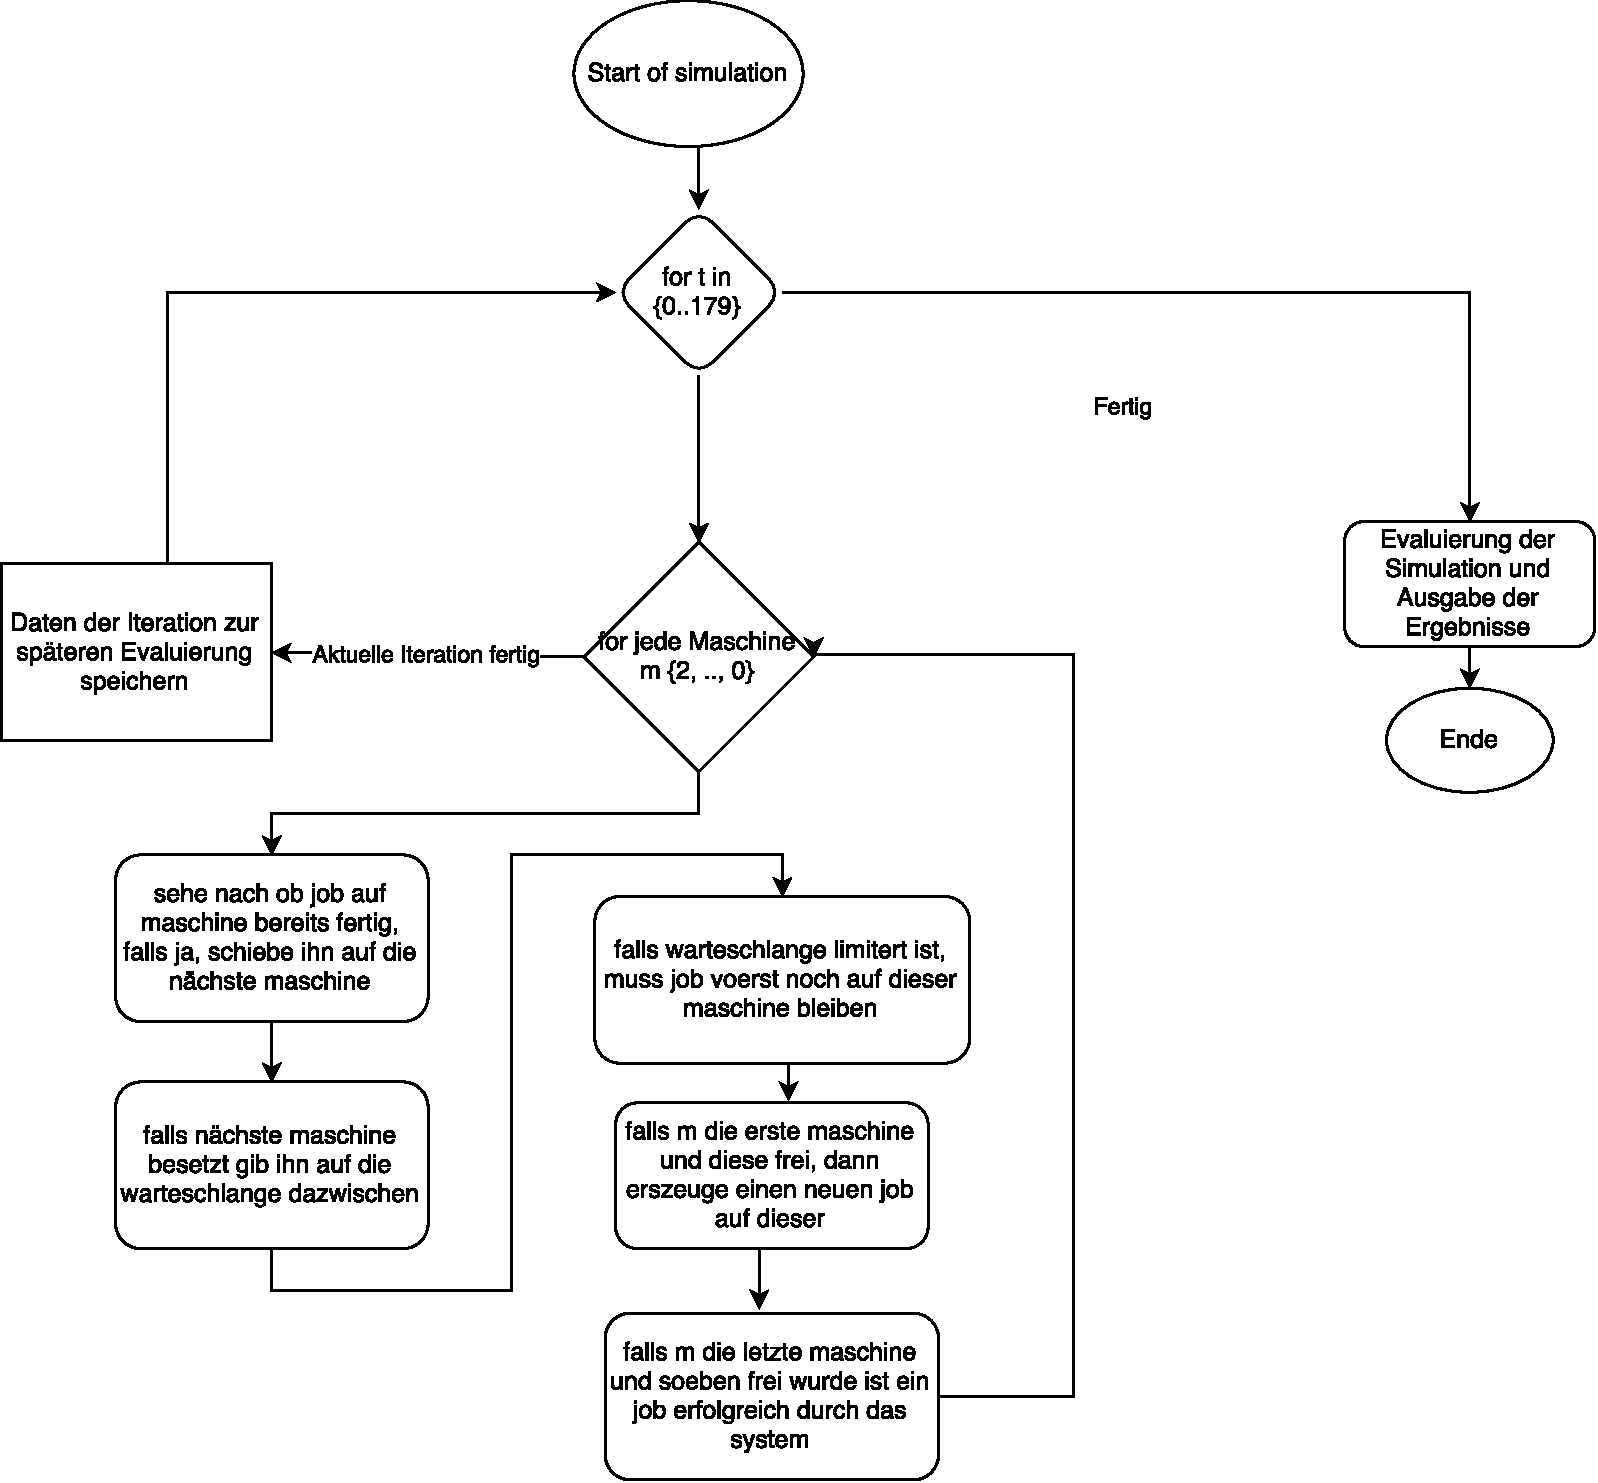
\includegraphics[scale=0.3]{BSP23_Flow_Chart.pdf}
\end{frame}

\subsection{Verwendete Funktionen}
\begin{frame}[fragile]{Funktion loaded\_random\_choice(..)}
  \begin{itemize}
    \item Diese Funktion verlangt eine WSKL Liste als Eingabeparameter
    \item Gibt einen Index zurück, welcher 0 bis $\left\vert{probality\_list}\right\vert-1$ sein kann.
    \item Diese Indizes haben eine gewichtete WSKL, welche jeweils an der Position in der Eingabeliste steht
    \item Beispiel probility\_list := [ 0.9, 0.1 ]  $\Rightarrow$ mit p=90\% wird 0 zurückgegeben, p=10\% für 1
  \end{itemize}
  \begin{lstlisting}[language=python]
def loaded_random_choice(probability_list):
    n = len(probability_list)
    random_number = random.random()
    cum_p = 0
    for i in range(n):
        cum_p += probability_list[i]
        if cum_p > random_number:
            return i
    return None
\end{lstlisting}
\logopythonbottom
\end{frame}	

\section{Grafische Darstellung}
\begin{frame}[fragile]{Gantt Diagramm - Zur Veranschaulichung des Unterschieds mit und ohne Zwischenpuffer}
\begin{center}
	\vspace{-.8cm}
  	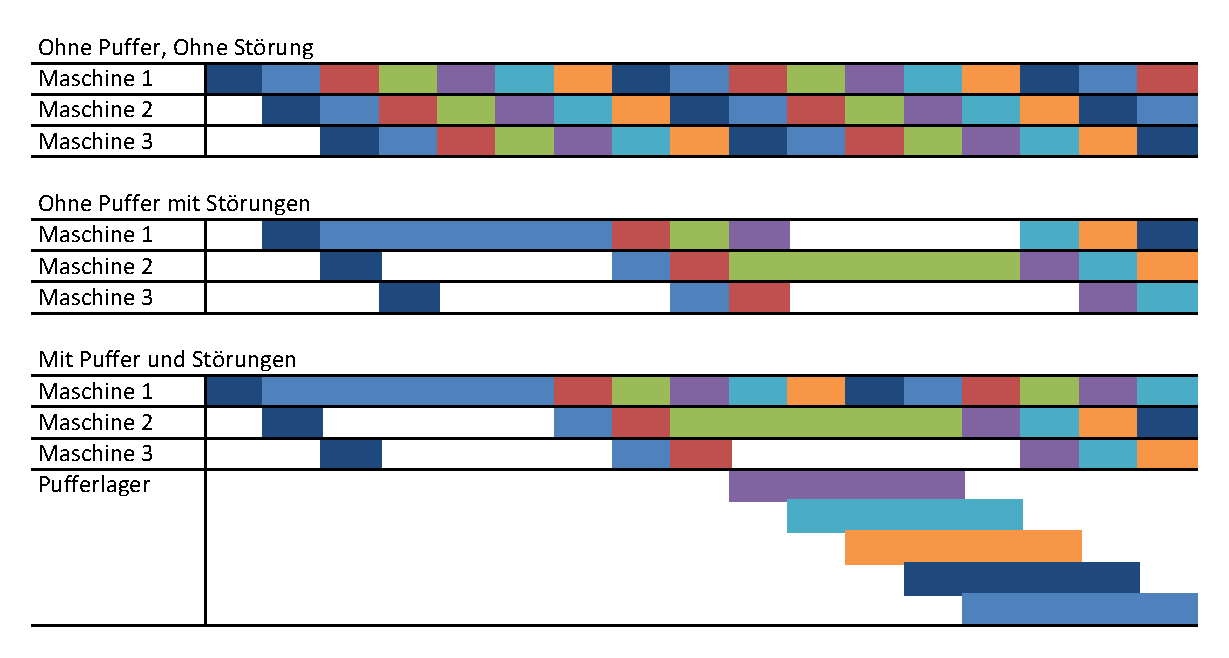
\includegraphics[scale=.6]{BSP23_Gantt.pdf}
\end{center}
\end{frame}

\end{document}
